\documentclass[12pt, twoside, openany]{book}
%\documentclass[12pt, oneside]{book}  % jednostranna tlac
\linespread{1.25} % hodnota 1.25 by mala zodpovedat 1.5 riadkovaniu
\pagestyle{plain}
% -------------------
% --- Packages
% -------------------
\usepackage[a4paper,top=2.5cm,bottom=2.5cm,left=3.5cm,right=2cm]{geometry}
\usepackage[utf8]{inputenc}
\usepackage[T1]{fontenc}
\usepackage{graphicx}
\usepackage{url}

% --- additional packages
\usepackage{epsfig}
\usepackage{epstopdf}
%\usepackage[chapter]{algorithm}
\usepackage{algorithmic}
%\usepackage{listings}
\usepackage{amsmath}
\usepackage{amssymb}
\usepackage{multirow}
\usepackage{booktabs}
\usepackage{color}
\usepackage{setspace}
\usepackage{tabularx}
\usepackage{textcomp}
\usepackage{caption}
\usepackage{natbib}
\usepackage{subcaption}
\usepackage[font=large]{subcaption}
\usepackage{emptypage}
\usepackage{float}
\usepackage[hidelinks,breaklinks]{hyperref}
\usepackage{minted}
\usepackage[thinlines]{easytable}
\usepackage{amsmath}

%\captionsetup[subfigure]{font=large}




%aby sa nevykreslovali obrazky
%\renewcommand{\includegraphics}[2][]{
%   \fbox{#2}% print file name in a small box
%}


% -------------------
% --- Definicia zakladnych pojmov
% -------------------
\def\mfrok{2025}
\def\mftitle{Exploring Translation and Reasoning Abilities of Large Language Models in the \v{S}aris Dialect}
\def\mfthesistype{Master thesis}
\def\mfauthor{Bc. Viktória Ondrejová}
\def\mfskolitel{Mgr. Marek Šuppa}
\def\mfplacedate{Bratislava, 2025}
\def\mfuniversity{COMENIUS UNIVERSITY IN BRATISLAVA}
\def\mffaculty{FACULTY OF MATHEMATICS PHYSICS AND INFORMATICS}
\def\mfodbor{Applied informatics}
\def\program{Applied informatics}
\def\mfpracovisko{Department of Applied Informatics }

\begin{document}
\frontmatter


% -------------------
% --- Obalka ------
% -------------------
\thispagestyle{empty}

\noindent
\begin{minipage}{\textwidth}
    \begin{center}
        \textbf{\mfuniversity \\
        \mffaculty}
    \end{center}
\end{minipage}

\vfill
\begin{figure}[!hbt]
	\begin{center}
		\includegraphics[width=0.4\textwidth]{images/UK_logo.png}
		\label{img:logo}
	\end{center}
\end{figure}
\begin{center}
		\textbf{\MakeUppercase{\Large\mftitle}}\\
		\mfthesistype
\end{center}
\vfill
\mfrok \hfill
\mfauthor
%\eject 
\cleardoublepage
% --- koniec obalky ----



% -------------------
% --- Titulný list
% -------------------
\thispagestyle{empty}
\noindent
\begin{minipage}{\textwidth}
    \begin{center}
        \textbf{\mfuniversity \\
        \mffaculty}
    \end{center}
\end{minipage}

\vfill
\begin{figure}[!hbt]
    \begin{center}
        \includegraphics[width=0.4\textwidth]{images/UK_logo.png}
        \label{img:logo_dark}
    \end{center}
\end{figure}

\begin{center}
	\textbf{\MakeUppercase{\Large\mftitle}}\\
	\mfthesistype
\end{center}
\vfill


\begin{tabular}{l l}
Study program: & \program \\
Branch of study: & \mfodbor \\
Department: & \mfpracovisko \\
Supervisor: & \mfskolitel \\
\end{tabular}

\vfill
\noindent
\mfplacedate \hfill
\mfauthor
%\eject 
\cleardoublepage
% --- Koniec titulnej strany



% -------------------
% --- Zadanie z AIS
% -------------------
% v tlačenej verzii s podpismi zainteresovaných osôb.
% v elektronickej verzii sa zverejňuje zadanie bez podpisov
% v pracach v naglictine anglicke aj slovenske zadanie

\newpage 
\thispagestyle{empty}
\hspace{-2cm}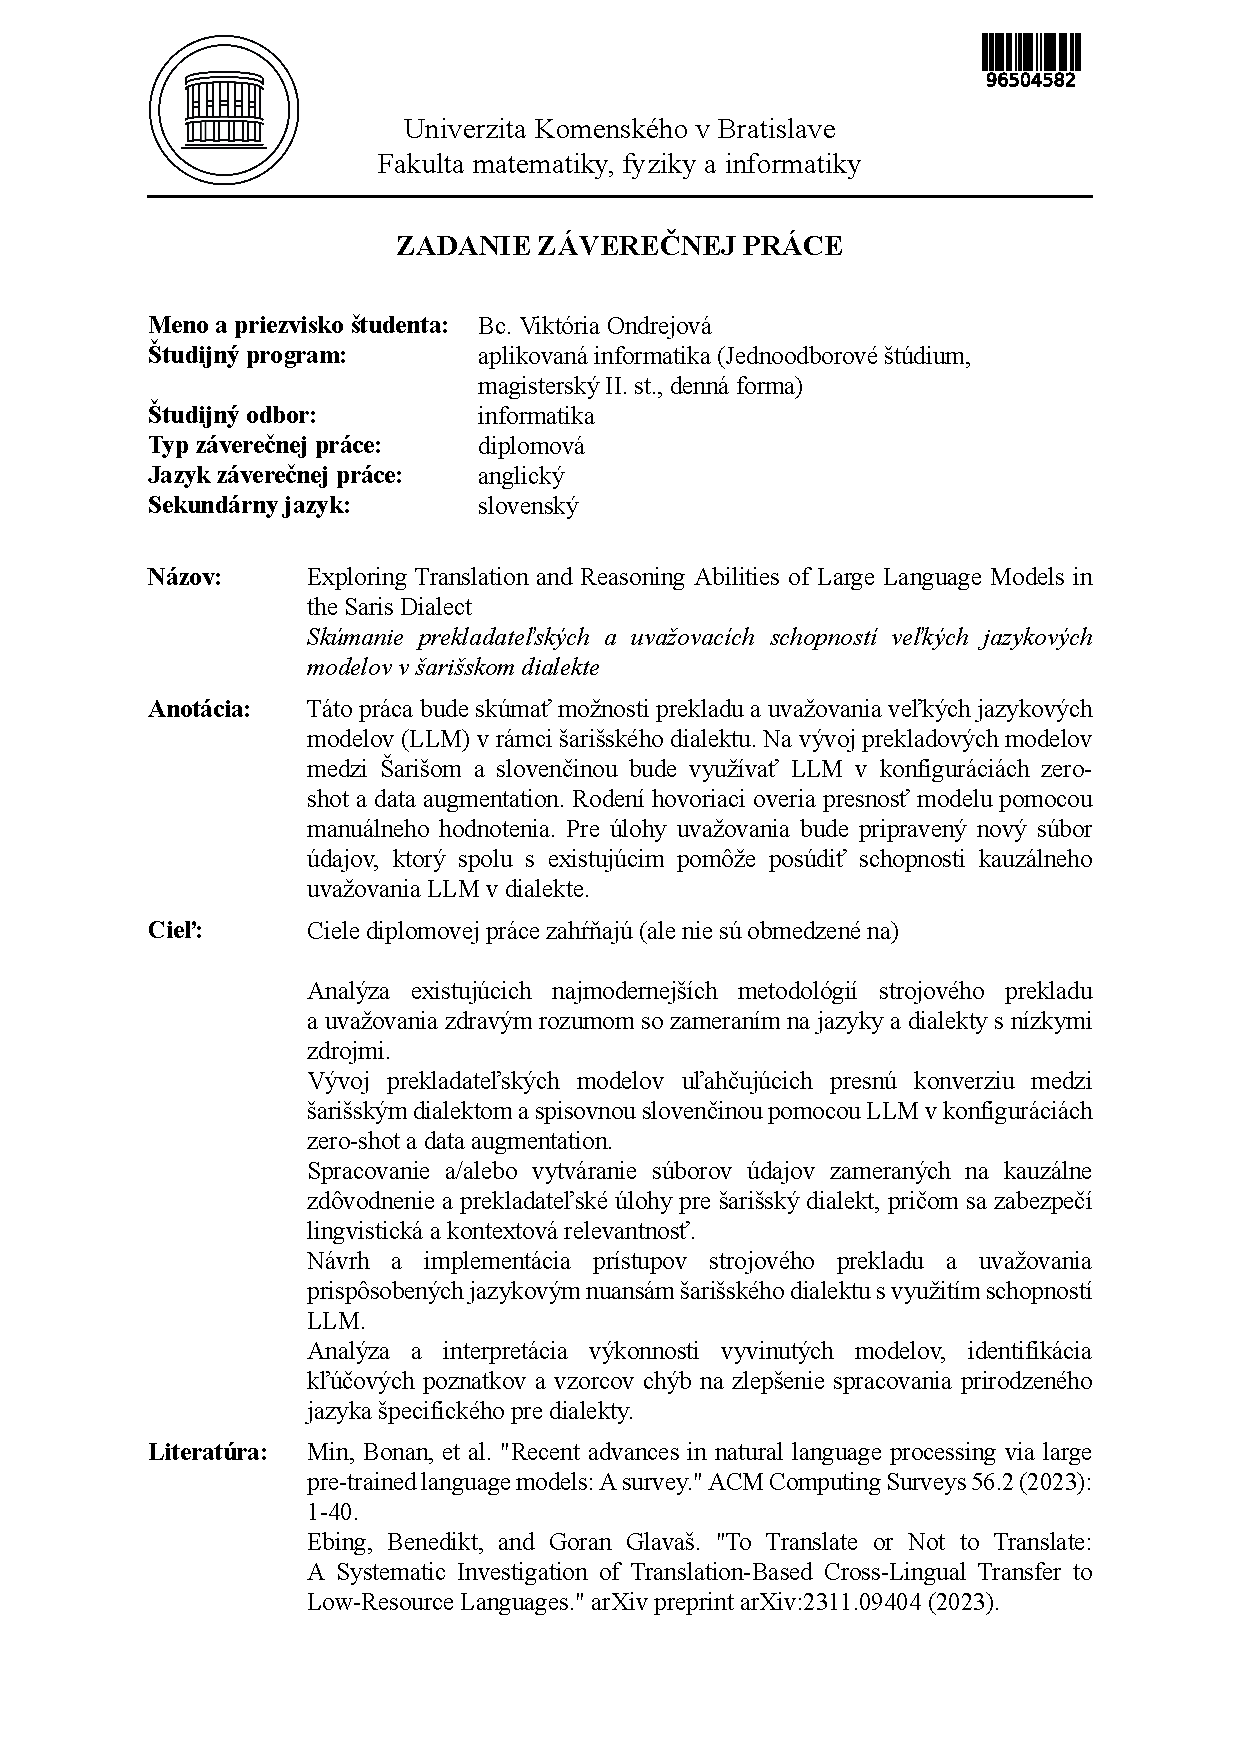
\includegraphics[page=1,width=1.1\textwidth]{zadaniePrace.PDF}

\newpage 
\thispagestyle{empty}
\hspace{-2cm}\includegraphics[page=2,width=1.1\textwidth]{zadaniePrace.PDF}

% --- Koniec zadania


% -------------------
% --- Prehlásenie
% -------------------

{~}\vspace{12cm}

\noindent
\begin{minipage}{0.25\textwidth}~\end{minipage}
\thispagestyle{empty}
\begin{minipage}{0.75\textwidth}
I hereby declare that I have written this thesis by myself, only with help of referenced literature, under the careful supervision of my thesis advisor.
\newline \newline
\end{minipage}
\vfill
~ \hfill {\hbox to 6cm{\dotfill}} \\
\mfplacedate \hfill \mfauthor
\vfill\eject \cleardoublepage
% --- koniec prehlasenia




% -------------------
% --- Poďakovanie
% -------------------
\newpage
\thispagestyle{empty}
\chapter*{Acknowledgement}\label{chap:thank_you}


\vfill\eject 
% --- koniec podakovania



% -------------------
% --- Abstrakty
% -------------------
\newpage 
\thispagestyle{empty}
\chapter*{Abstract}\label{chap:abstract_en}
\input{abstract}

\paragraph*{Keywords: NLP, LLM, low-resource languages, dialect}  


\newpage 
\thispagestyle{empty}
\chapter*{Abstrakt}\label{chap:abstract_sk}



\paragraph*{Kľúčové slová: NLP, LLM, jazyky s málo dátami, dialekt}


% --- koniec abstraktov


% -------------------
% --- Obsah
% -------------------
\newpage 
\tableofcontents

% ---  Koniec Obsahu


\newpage 
\input{terminology}
\newpage 
\chapter{Introduction}
\chapter{Related Work}
\input{saris}
\chapter{Data}
\chapter{Experiments}
\newpage
\chapter{Evaluation}
\chapter{Results}


\mainmatter




%main content 


% -------------------
% --- Bibliografia
% -------------------

\backmatter

\nocite{*}
\bibliographystyle{plain}
\bibliography{references}

%---koniec bibliografie

\end{document}